\section{风生洋流的匀质模式}

\subsection{大洋环流的基本特征}

大尺度大洋环流按照深度和驱动机制可分为\textbf{表层环流}和\textbf{深层环流}两类。

\subsubsection{表层环流 (Surface Circulation)}

表层环流主要分布在大洋上层约 $1000\,\mathrm{m}$ 的区域，是由大气风场直接驱动的\textbf{风生洋流}。
风应力通过摩擦作用将动量传递给海洋表层，形成大规模的水平环流系统。
图 \ref{fig:global_ocean_currents_nasa} 展示了基于卫星观测数据的全球表层环流分布。

\begin{figure}[htbp]
    \centering
    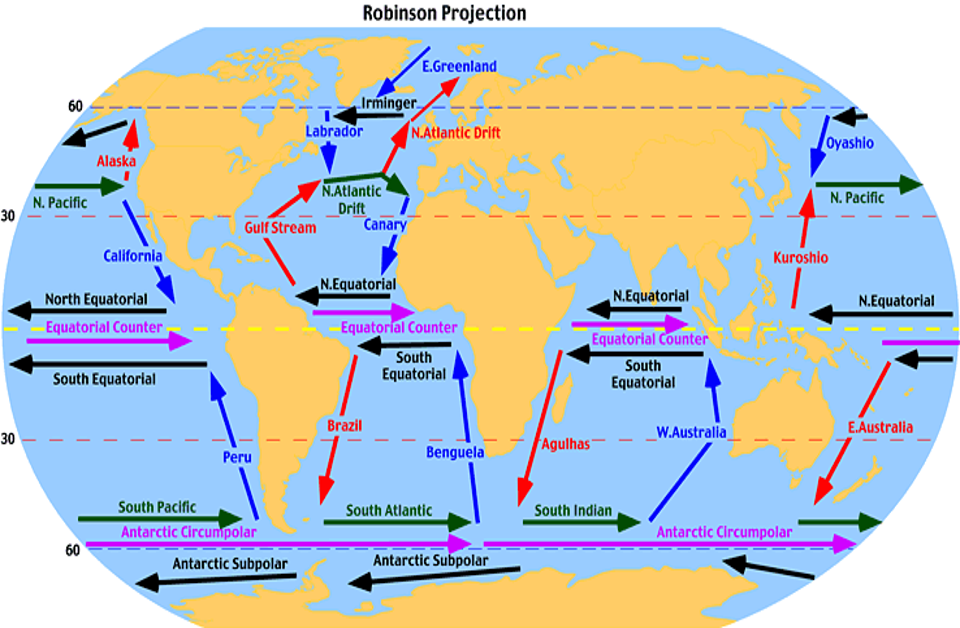
\includegraphics[width=1.00\textwidth]{assets/global_ocean_currents_nasa.png}
    \caption{全球表层环流分布图 (数据来源: NASA Goddard Space Flight Center)}
    \label{fig:global_ocean_currents_nasa}
\end{figure}

大洋表层环流呈现以下显著特征:

\textbf{(i) 对风向转换的响应}

表层环流的旋转方向与大气环流的风向分布密切相关: 北半球环流沿顺时针方向流动；南半球环流沿逆时针方向流动。
这一特征与大气环流的纬向风分布相对应: 中纬度为西风带，低纬度为东风带 (信风带)。
风应力在副热带海域形成负的风应力旋度，驱动反气旋式环流。

\textbf{(ii) 东西边界的不对称性——西部强化}

大洋环流在东西边界附近呈现显著的不对称性，即\textbf{西部强化}。
大洋环流的一般流速约为 $1\text{--}10\,\mathrm{cm/s}$；
西边界流 (如黑潮、湾流) 流速可达 $100\text{--}200\,\mathrm{cm/s}$，较东边界流强一个量级以上。

\textbf{(iii) 中尺度涡旋 (Mesoscale Eddies)}

大洋中广泛存在水平特征尺度为 $1\text{--}500\,\mathrm{km}$，垂直特征尺度为数米至数百米的中尺度涡旋结构。
中尺度涡旋是海洋中能量最为集中的运动形式之一，对海洋物质输运和能量级联有重要影响。
针对海洋中尺度涡旋的基础理论、观测、数值模拟及其环境效应研究，是当前海洋科学研究的重要前沿。

\subsubsection{深层环流 (Deep Circulation)}

深层环流，又称\textbf{温盐环流 (Thermohaline Circulation, THC)}，是依靠海水的温度和盐度差异驱动的全球洋流循环。
其基本机制为: 在高纬度海域，海水因低温和高盐度而具有较大的密度，在重力作用下下沉至深层，沿等密度面向低纬度流动；
而在低纬度海域，密度较小的暖水团则会上涌并向高纬度流动，由此形成全球尺度的闭合环流。

温盐环流在全球气候系统中发挥着至关重要的作用，是低纬度向高纬度输送热量的重要载体，对维持地球热量平衡起着关键作用。
温盐环流的改变及其伴随的极向热输送变化，会对局地和全球气候产生重大影响。

IPCC第六次评估报告 (AR6) 指出，\textbf{大西洋经向翻转环流 (Atlantic Meridional Overturning Circulation, AMOC)} 在2000年代中期至2010年代中期有所减弱。
一旦AMOC发生崩溃，将导致天气模式和水循环的剧烈变化，如热带雨带南移、非洲和亚洲的季风减弱等。

\subsection{匀质模式 (Homogeneous Model)}

在本章中，我们将主要讨论表层环流 (风生洋流) 的动力学特征。
为此，我们建立一个理想化的\textbf{匀质大洋模型}。
该模型试图通过一个“统一解”，将自由面边界层、底部边界层以及深厚内区的运动规律联系起来。

考虑一个大洋盆地，特征尺度为:
\begin{itemize}
    \item \textbf{水平长度尺度}: $\hscale$ (大洋盆地宽度)；
    \item \textbf{垂直长度尺度}: $\vscale$ (大洋平均深度)；
    \item \textbf{水平速度尺度}: $\hvel$ (大洋环流典型流速)。
\end{itemize}

我们将流体运动分解为三个区域:
\begin{itemize}
    \item \textbf{表层}: 受风应力 $\wind$ 直接驱动的薄摩擦层。
    \item \textbf{内区}: 远离边界，近似满足地转平衡的深厚区域。
    \item \textbf{底层}: 受海底摩擦影响的薄摩擦层。
\end{itemize}

为了简化数学处理，我们引入以下核心假设:
\begin{enumerate}
    \item \textbf{密度均匀且不可压缩}: 假设海水密度均匀，即密度 $\density$ 是一个常数。
    这意味着我们忽略斜压效应，且不考虑层结。
    连续性方程简化为不可压缩条件 $\nabla \cdot \vel = 0$。
    \item \textbf{平坦海底}: 假设海底地形平坦，$\bottomheight = 0$。
    \item \textbf{刚盖近似}: 自由面平坦，忽略海面高程变化对流体运动的影响。
    \item \textbf{风驱动}: 海洋运动完全归因于海面风应力的驱动，忽略热盐环流因素。
\end{enumerate}

在以上假设下，边界条件为:
\begin{itemize}
    \item \textbf{海底} (无滑移条件):
    \begin{equation}
        \vel = \ivec{0}
        \label{eq:ocean_boundary_condition_top}
    \end{equation}
    \item \textbf{海面} (风应力平衡):
    \begin{equation}
        \density \eddyviscv \pde{\vel_h}{z} = \wind
        \label{eq:ocean_boundary_condition_bottom}
    \end{equation}
\end{itemize}

控制方程为雷诺平均方程 \eqref{eq:rans_closed}。

\subsubsection{无量纲化}

进行尺度分析。
由连续性方程 $\nabla \cdot \vel = 0$，垂直速度的量级为 $\vvel = \frac{\hvel \vscale}{\hscale}$。
时间尺度取平流时间尺度 $\timescale = \hscale / \hvel$。
在大尺度地球流体中，科里奥利力远远大于惯性力，因此水平方向上压力梯度力主要用于抵消科里奥利力的影响，二者量级相当。
因此，$\pressure \sim -\density \gravityconst z + \density \coriolis \hvel \hscale$。

方程 \eqref{eq:rans_closed} 的各项量级如下:
\begin{align*}
    \underbrace{\pde{\vel_h}{\timevar}}_{\hvel^2 / \hscale} + \underbrace{(\vel \cdot \nabla) \vel_h}_{\hvel^2 / \hscale} &= -\underbrace{\coriolis \kvec \times \vel_h}_{\coriolis \hvel} - \underbrace{\frac{1}{\density} \nabla_h \pressure}_{-\coriolis \hvel} + \underbrace{\eddyvisch \nabla_h^2 \vel_h}_{\eddyvisch \hvel / \hscale^2} + \underbrace{\eddyviscv \nabla_z^2 \vel_h}_{\eddyviscv \hvel / \vscale^2} \\
    \underbrace{\pde{w}{\timevar}}_{\hvel^2 \vscale / \hscale^2} + \underbrace{(\vel \cdot \nabla) w}_{\hvel^2 \vscale / \hscale^2} &= \underbrace{-\frac{1}{\density} \pde{\pressure}{z}}_{\gravityconst - \coriolis \hvel \hscale / \vscale} - \gravityconst + \underbrace{\eddyvisch \nabla_h^2 w}_{\eddyvisch \hvel \vscale / \hscale^3} + \underbrace{\eddyviscv \nabla_z^2 w}_{\eddyvisch \hvel / \vscale \hscale}
\end{align*}

得到无量纲的雷诺平均方程:
\begin{align}
    \ro \matderiv{\vel_h} &= -\kvec \times \vel_h -\nabla_h p_ + \frac{\eh}{2} \nabla_h^2 \vel_h + \frac{\ev}{2} \nabla_z^2 \vel_h \label{eq:rans_nondim_h} \\
    \vhratio^2 \ro \matderiv{w} &= -\pde{p}{z} + \vhratio^2 \left(\frac{\eh}{2} \nabla_h^2 w + \frac{\ev}{2} \nabla_z^2 w\right) \label{eq:rans_nondim_v}
\end{align}

其中出现了四个重要的无量纲参数:
\begin{enumerate}
    \item \textbf{Rossby数}: $\ro = \frac{\hvel}{\coriolis \hscale}$，表征惯性力与科里奥利力的比值。
    在大尺度大洋环流中，$\ro \ll 1$，说明非线性平流项通常是次要的。

    \item \textbf{形态比}: $\vhratio = \frac{\vscale}{\hscale} \ll 1$，表征垂直尺度与水平尺度的比值。

    \item \textbf{水平Ekman数}: $\eh = \frac{2\eddyvisch}{\coriolis \hscale^2}$，表征水平摩擦力与科里奥利力的比值。

    \item \textbf{垂直Ekman数}: $\ev = \frac{2\eddyviscv}{\coriolis \vscale^2}$，表征垂直摩擦力与科里奥利力的比值。
    Ekman深度 $\ekmandepth = \sqrt{2\eddyviscv/\coriolis}$，因此 $\ev = (\ekmandepth / \vscale)^2$。
    由于 $\ekmandepth \ll \vscale$，$\ev \ll 1$。
\end{enumerate}

为了直观认识上述参数的量级，我们选取中纬度大洋环流的典型特征尺度进行估算:
水平尺度 $\hscale \sim 10^6\,\mathrm{m}$；垂直尺度 $\vscale \sim 10^3\,\mathrm{m}$；水平速度 $\hvel \sim 10^{-2}\,\mathrm{m/s}$，
科里奥利参数 $\coriolis \sim 10^{-4}\,\mathrm{s^{-1}}$。
涡粘系数的不确定性较大，取 $\eddyvisch = 10^2 \text{--} 10^3 \mathrm{m^2/s}$，$\eddyviscv \sim 10^{-3} \text{--} 10^{-2} \mathrm{m^2/s}$

代入计算可得无量纲参数的典型值:
\begin{itemize}
    \item $\ro \sim 10^{-4}$
    \item $\vhratio \sim 10^{-3}$
    \item $\eh \sim 10^{-6} \text{--} 10^{-5}$
    \item $\ev \sim 10^{-5} \text{--} 10^{-4}$ (对应Ekman深度 $\ekmandepth \sim 4.5\,\mathrm{m}$)
\end{itemize}

\subsubsection{摄动法 (Perturbation Method)}

我们使用\textbf{摄动法} 求解非线性偏微分方程组。
摄动法，又称小参数法或WKBJ方法，其核心思想是将方程关于某个合适的小参数 (摄动量) 作幂级数展开，求各级渐进解。

观察方程 \eqref{eq:rans_nondim_h}，\eqref{eq:rans_nondim_v}，其中包含四个小参数: $\ro, \vhratio, \eh, \ev$。
在大尺度大洋环流中，这些参数均远小于 $1$。
我们选取其中量级最大者作为摄动小参数 $\Delta$，其中$\Delta = \Delta(\ro, \vhratio, \eh, \ev) \sim \ro \sim \vhratio$。
将物理量展开为关于 $\Delta$ 的幂级数:
\begin{equation}
    \wavefunc(\pos, \timevar, \ro, \vhratio, \eh, \ev) = \sum_{n=0}^{\infty} \frac{1}{n!} \Delta^n(\ro, \vhratio, \eh, \ev) \wavefunc_n(\pos, \timevar)
    \label{eq:perturbation_expansion}
\end{equation}

将展开式代入原方程，令 $\Delta$ 的同次幂系数之和为零，即得到各级近似方程，从而可以逐级求解。

\subsubsection{内区解 (Interior Solution)}

我们首先讨论远离边界层的内区流体运动特征。

对于零阶项，非线性项 ($\ro$) 和摩擦项 ($\eh, \ev$) 均被忽略。
零阶近似下的水平动量方程 \eqref{eq:rans_nondim_h} 退化为\textbf{地转平衡}关系，垂直动量方程 \eqref{eq:rans_nondim_h} 退化为\textbf{静力平衡}关系:
\begin{align}
    \kvec \times \vel_{h0} &= -\nabla_{h} \pressure_0 \label{eq:interior_geostrophic} \\
    \pde{\pressure_0}{z} &= 0 \label{eq:interior_hydrostatic}
\end{align}

结合两式，得到\textbf{Taylor-Proudman定理}:
\begin{equation}
    \pde{\vel_{h0}}{z} = 0
    \label{eq:interior_taylor_proudman}
\end{equation}

这表明在匀质大洋内区，\textbf{零阶水平速度与深度无关}，流体以刚柱形式运动。

对 \eqref{eq:interior_geostrophic} 应用水平旋度算子:
\begin{equation}
    \nabla_h \cdot \vel_{h0} = \kvec \cdot (\nabla_h \times (\kvec \times \vel_{h0})) = -\kvec \cdot \nabla_h \times \nabla_h \pressure_0 = 0
    \label{eq:interior_continuity}
\end{equation}

而连续性方程为 $\nabla \cdot \vel_0 = 0$，因此 $\pde{w_0}{z} = 0$。
这说明匀质大洋内区，\textbf{零阶垂直速度为常数}。

零阶近似下的解表征的是\textbf{内区的地转运动特征}，是远离边界层的大洋环流的基本运动规律。
它是当 $\ro, \vhratio, \eh, \ev \to 0$ 时的极限解，相当于忽略了相对加速度项、水平扩散项以及摩擦项。
对于实际的内区流体运动，我们还必须考虑非地转运动 (地转偏差)，这需要计算更高阶的近似作为修正。

根据 \eqref{eq:interior_taylor_proudman}，$\frac{\ev}{2} \nabla_z^2 \vel_{h0} = 0$，这意味着垂直摩擦项对内区零阶流场不产生作用。
引入水平雷诺数 $(\re)_H = \frac{\hvel \hscale}{\eddyvisch}$，我们考察关于小参数 $\Delta$ 的一阶近似。
将展开式代入方程 \eqref{eq:rans_nondim_h}，收集一阶项:
\begin{equation*}
    \matderiv{\vel_{h0}} = -\kvec \times \vel_{h1} - \nabla_h \pressure_1 + \frac{1}{(\re)_H} \nabla_h^2 \vel_{h0}
\end{equation*}

为消除一阶压力项 $\pressure_1$，我们对上式应用水平旋度算子:
\begin{itemize}
    \item 根据 \eqref{eq:interior_continuity} 和涡旋拉伸效应 \eqref{eq:vortex_stretching_proof}，左式整理为:
    \begin{equation*}
        \kvec \cdot \left(\nabla_h \times \matderiv{\vel_{h0}}\right) = \matderiv{\relvort_0} + \relvort_0 (\nabla_h \cdot \vel_{h0}) = \matderiv{\relvort_0}
    \end{equation*}

    \item 标量场梯度的旋度恒为零，根据连续性条件，右式整理为:
    \begin{align*}
        \kvec \cdot \left[\nabla_h \times \left(-\kvec \times \vel_{h1} - \nabla_h \pressure_1 + \frac{1}{(\re)_H} \nabla_h^2 \vel_{h0}\right)\right] &= -\nabla_h \cdot \vel_{h1} + \frac{1}{(\re)_H} \nabla_h^2 \relvort_0 \\
        &= \pde{w_1}{z} + \frac{1}{(\re)_H} \nabla_h^2 \relvort_0
    \end{align*}
\end{itemize}

综上，得到\textbf{准地转涡度方程}:
\begin{equation}
    \matderiv{\relvort_0} = \pde{w_1}{z} + \frac{1}{(\re)_H} \nabla_h^2 \relvort_0
    \label{eq:qg_vorticity_nondim}
\end{equation}

恢复为有量纲形式，其中 $w_1 \sim w_0 / \ro$:
\begin{equation}
    \matderiv{\relvort_0} = \coriolis \pde{w_0}{z} + \eddyvisch \nabla_h^2 \relvort_0
    \label{eq:qg_vorticity}
\end{equation}

准地转涡度方程揭示了内区流体相对涡度变化的两种主要机制:
\begin{enumerate}
    \item \textbf{涡管伸缩 (Vortex Stretching)} $\coriolis \pde{w_0}{z}$:
    当流体柱在垂直方向被拉伸时，根据角动量守恒，其水平截面积减小，旋转角速度 (涡度) 必须增加。
    这建立了垂直运动与水平环流之间的动力学联系。

    \item \textbf{湍流水平扩散} $\eddyvisch \nabla_h^2 \relvort_0$:
    表示涡度由于水平湍流混合而发生的耗散，使涡度场趋于均匀化。
\end{enumerate}

\subsection{风生洋流 (Wind-driven Circulation)}

\subsubsection{底部边界层}

在底部边界层内，流体速度 $\vel$ 必须在一个比大洋深度 $\vscale$ 小得多的垂直尺度上发生剧烈变化，使摩擦项足以成为局部的重要因子。
为研究这一薄层内的动力学，我们引入\textbf{伸缩坐标}:
\begin{equation}
    \xi = \frac{z}{l}
    \label{eq:stretched_coordinate_bottom}
\end{equation}

其中 $l$ 是待定的边界层特征厚度。

在新坐标下，垂直导数变换为:
\begin{equation}
    \pde{}{z} = \frac{1}{l} \pde{}{\xi}
    \label{eq:vertical_derivative_transform_bottom}
\end{equation}

特征厚度 $l$ 的选取准则是使垂直摩擦力与科里奥利力在量级上相当:
\begin{equation*}
    \frac{\eddyviscv \hvel}{l^2} \sim \coriolis \hvel \implies l \sim \sqrt{\frac{\eddyviscv}{\coriolis}} = \frac{\ekmandepth}{\sqrt{2}} \sim \vscale \ev^{1/2}
\end{equation*}

因此，底部边界层内的无量纲雷诺平均方程变为:
\begin{align}
    \ro (\flayer{\vel_h} \cdot \nabla_h) \flayer{\vel_h} + \frac{\ro}{\ev^{1/2}} (\flayer{\vel_\xi} \cdot \nabla_\xi) \flayer{\vel_h} &= -\kvec \times \flayer{\vel_h} -\nabla_h \flayer{\pressure} + \frac{\eh}{2} \nabla_h^2 \flayer{\vel_h} + \frac{1}{2} \nabla_\xi^2 \flayer{\vel_h} \label{eq:rans_nondim_h_boundary_bottom} \\
    \vhratio^2 \left(\ro (\flayer{\vel_h} \cdot \nabla_h) \flayer{w} + \frac{\ro}{\ev^{1/2}} (\flayer{\vel_\xi} \cdot \nabla_\xi) \flayer{w}\right) &= -\frac{1}{\ev^{1/2}} \pde{\flayer{\pressure}}{\xi} + \vhratio^2 \left(\frac{\eh}{2} \nabla_h^2 \flayer{w} + \frac{1}{2} \nabla_\xi^2 \flayer{w}\right) \label{eq:rans_nondim_v_boundary_bottom}
\end{align}

考虑零阶近似:
\begin{align}
    -\kvec \times \flayer{\vel_{h0}} -\nabla_h \flayer{\pressure_0} + \frac{1}{2} \nabla_\xi^2 \flayer{\vel_{h0}} &= 0 \label{eq:momentum_boundary_bottom} \\
    \pde{\flayer{\pressure_0}}{\xi} &= 0 \label{eq:hydrostatic_boundary_bottom}
\end{align}

其中 \eqref{eq:hydrostatic_boundary_bottom} 表明底部边界层内在垂直方向上仍满足静力平衡。
这意味着底部边界层内的水平压力梯度与内区相同，可以用内区的地转关系表示:
\begin{equation*}
    -\nabla_h \flayer{\pressure_0} = -\nabla_{h} \pressure_0 = \kvec \times \vel_{h0}
\end{equation*}

代入 \eqref{eq:rans_nondim_h_boundary_bottom}:
\begin{equation*}
    \frac{1}{2} \pde[2]{\flayer{\vel_{h0}}}{\xi} -\kvec \times \flayer{\vel_{h0}} = -\kvec \times \vel_{h0}
\end{equation*}

边界条件为:
\begin{itemize}
    \item \textbf{上边界} (匹配内区解): $\flayer{\vel_{0}}(\infty) = \vel_{0}$。
    \item \textbf{下边界} (无滑移条件): $\flayer{\vel_{0}}(0) = \ivec{0}$。
\end{itemize}

注意到，方程形式与Ekman平衡方程 \eqref{eq:ekman_equation} 一致，且具有相同的边界条件。
因此，底部边界层实际上正是经典的Ekman层，方程解所描述的速度场为Ekman螺线。

直接写出底部边界层内的速度分布:
\begin{equation}
    \complex{\flayer{\vel_{h0}}}(\xi) = \complex{\vel_{h0}} (1 - e^{-(1+i) \xi})
    \label{eq:solution_complex_boundary_bottom}
\end{equation}

矢量形式为:
\begin{equation}
    \flayer{\vel_{h0}}(\xi) = \vel_{h0}(1 - e^{-\xi} \cos\xi) + (\kvec \times \vel_{h0}) e^{-\xi} \sin\xi
    \label{eq:solution_boundary_bottom}
\end{equation}

\subsubsection{自由面边界层}

对于自由面边界层，摩擦项同样是局部的重要因子。
引入以自由面为原点的伸缩坐标:
\begin{equation}
    \varsigma = \frac{z - \vscale}{l}
    \label{eq:stretched_coordinate_top}
\end{equation}

其中 $l = \frac{\ekmandepth}{\sqrt{2}}$ 为边界层特征厚度。
$\varsigma = 0$ 对应自由面，$\varsigma \to -\infty$ 对应内区。

关于 $\varsigma$ 的垂直导数变换和 $\xi$ 完全一致:
\begin{equation}
    \pde{}{z} = \frac{1}{l} \pde{}{\varsigma}
    \label{eq:vertical_derivative_transform_top}
\end{equation}

因此，自由面边界层内的无量纲平均方程与底部边界层形式一致: \eqref{eq:rans_nondim_h_boundary_bottom}，\eqref{eq:rans_nondim_v_boundary_bottom}。
在零阶近似下可导出相同的控制方程:
\begin{equation*}
    \frac{1}{2} \pde[2]{\flayer{\vel_{h0}}}{\varsigma} -\kvec \times \flayer{\vel_{h0}} = -\kvec \times \vel_{h0}
\end{equation*}

边界条件为:
\begin{itemize}
    \item \textbf{上边界} (应力连续条件):
    有量纲形式为 $\left.\density \eddyviscv \pde{\flayer{\vel_{h0}}}{\varsigma}\right|_{\varsigma = 0} = \wind$。

    设特征风应力强度为 $\tau$，定义无量纲风应力参数 $\alpha = \frac{\vscale \ev^{1/2} \tau}{\sqrt{2} \density \eddyviscv \hvel} = \frac{\ekmandepth \tau}{\sqrt{2} \density \eddyviscv \hvel} = \frac{1}{\hvel} \frac{\tau}{\density \sqrt{\coriolis \eddyviscv}}$。

    进行进行尺度分析，各项量级如下:
    \begin{equation*}
        \underbrace{\left.\density \eddyviscv \pde{\flayer{\vel_{h0}}}{\varsigma}\right|_{\varsigma = 0}}_{\density \eddyviscv \hvel / \vscale \ev^{1/2}} = \underbrace{\wind}_{\tau}
    \end{equation*}

    无量纲化的上边界条件为:
    \begin{equation*}
        \left.\pde{\flayer{\vel_{h0}}}{\varsigma}\right|_{\varsigma = 0} = \sqrt{2} \alpha \wind
    \end{equation*}

    \item \textbf{下边界} (匹配内区解): $\flayer{w_{h0}}(\varsigma \to -\infty) = \vel_{0}$。
\end{itemize}

注意到，控制方程与边界条件描述的实际上正是自由面Ekman层。
直接写出自由面边界层内的速度分布:
\begin{equation}
    \complex{\flayer{\vel_{h0}}}(\varsigma) = \complex{\vel_{h0}} + \alpha \complex{\wind} e^{\varsigma} \complexexp{\left(\varsigma - \frac{\pi}{4}\right)}
    \label{eq:solution_complex_boundary_top}
\end{equation}

在海面 ($\varsigma=0$) 处，Ekman漂流为:
\begin{equation}
    \complex{\flayer{\vel_{h0}}}(0) - \complex{\vel_{h0}} = \alpha \complex{\wind} \complexexpminus{\pi/4}
    \label{eq:surface_velocity_boundary_top}
\end{equation}

这说明海面Ekman漂流速度的大小与风应力成正比，方向相对于风应力矢量顺时针偏转 $45^\circ$ (在北半球)。

\subsubsection{Ekman抽吸 (Ekman Pumping)}

对于风生洋流问题，我们关注边界层摩擦引起的质量输运。
由于摩擦破坏了地转平衡，边界层内产生指向低压侧的跨等压线Ekman输运。
这种水平输运将通过连续性方程诱发垂直运动，即\textbf{Ekman抽吸}，进而通过涡管伸缩机制显著影响内区流场的演变。
Ekman抽吸是连接边界层与内区动力学的关键机制。

\textbf{(i) 底部边界层}

由连续性方程:
\begin{equation}
    \pde{\flayer{w_0}}{z} = \nabla_h \cdot \flayer{\vel_{h0}}
    \label{eq:continuity_boundary_layer}
\end{equation}

对 \eqref{eq:continuity_boundary_layer} 从 $z = 0$ 积分到 $z = \infty$:
\begin{itemize}
    \item 根据底部边界层的边界条件，左式:
    \begin{equation*}
        \int_0^\infty \pde{\flayer{w_0}}{z} \dd{z} = \flayer{w_0}(\infty) - \flayer{w_0}(0) = w_0
    \end{equation*}

    \item 根据 \eqref{eq:interior_continuity}，右式实际上正是Ekman输运 $\ekmantransport$ 的散度:
    \begin{equation*}
        \int_0^\infty (\nabla_h \cdot \flayer{\vel_{h0}}) \dd{z} = \int_0^\infty (\nabla_h \cdot (\flayer{\vel_{h0}} - \vel_{h0})) \dd{z} = \nabla_h \cdot \int_0^\infty (\flayer{\vel_{h0}} - \vel_{h0}) \dd{z} = \nabla_h \cdot \ekmantransport
    \end{equation*}
\end{itemize}

因此有 $w_0 = \nabla_h \cdot \ekmantransport$。
代入 \eqref{eq:ekman_transport_vector}:
\begin{align*}
    w_0 = \nabla_h \cdot \ekmantransport = \nabla_h \cdot \left(\frac{\ekmandepth}{2} (-\vel_{h0} + \kvec \times \vel_{h0})\right) &= \frac{\ekmandepth}{2} (-\nabla_h \cdot \vel_{h0} + \nabla_h \cdot (\kvec \times \vel_{h0})) \\
    &= \frac{\ekmandepth}{2} \kvec \cdot (\nabla_h \times \vel_{h0}) \\
    &= \frac{\ekmandepth}{2} \relvort_0
\end{align*}

综上，得到底部边界层的\textbf{Ekman抽吸公式}:
\begin{equation}
    w_0 = \frac{\ekmandepth}{2} \relvort_0
    \label{eq:ekman_pumping}
\end{equation}

该公式揭示了底部摩擦对内区流场的反馈机制。
当内区存在相对涡度 $\relvort_0$ 时，底部边界层内的摩擦作用会破坏地转平衡，产生跨等压线的质量输运。

\begin{itemize}
    \item \textbf{气旋式涡度 ($\relvort_0 > 0$)}: 对应低压中心。
    底部Ekman输运指向低压中心，产生质量辐合，迫使流体向上运动 ($w_0 > 0$)，形成\textbf{上升流}。
    \item \textbf{反气旋式涡度 ($\relvort_0 < 0$)}: 对应高压中心。
    底部Ekman输运背离高压中心，产生质量辐散，上方流体向下沉降 ($w_0 < 0$)，形成\textbf{下沉流}。
\end{itemize}

\textbf{(ii) 自由面边界层}

对 \eqref{eq:continuity_boundary_layer} 从 $z = -\infty$ 积分到 $z = 0$。
与底部边界层的推导类似，可得 $w_0 = \nabla_h \cdot \ekmantransport$。

代入 \eqref{eq:ekman_fs_transport}:
\begin{equation*}
    w_0 = \nabla_h \cdot \left(-\frac{1}{\density \coriolis} \kvec \times \wind\right) = \frac{1}{\density \coriolis} (\kvec \cdot (\nabla_h \times \wind))
\end{equation*}

得到自由面边界层的\textbf{Ekman抽吸公式}:
\begin{equation}
    w_0 = \frac{1}{\density \coriolis} (\kvec \cdot (\nabla_h \times \wind))
    \label{eq:ekman_pumping_fs}
\end{equation}

这说明风应力的旋度直接决定了海洋表层的垂直运动，是风生洋流的关键机制。

\begin{itemize}
    \item \textbf{气旋式风应力 ($\wind$ 的水平旋度为正)}: 产生表面Ekman输运的辐散。
    为填补表层流失的海水，深层海水上涌补充 ($w_0 > 0$)，形成“抽吸”。
    \item \textbf{反气旋式风应力 ($\wind$ 的水平旋度为负)}: 产生表面Ekman输运的辐合。
    堆积的海水迫使表层流体向下沉降 ($w_0 < 0$)，形成“泵压”。
\end{itemize}

\begin{insightbox}[风生洋流匀质模式的物理图景]
    \begin{enumerate}
        \item \textbf{内区与边界层的渐近结构}:
        匀质大洋环流在数学上表现为奇异摄动问题，流场被分解为深厚的内区和两个薄的摩擦边界层。
        内区由准二维、准水平、准地转的无粘动力学主导，而边界层则负责通过摩擦项诱导系统满足边界条件。

        \item \textbf{Ekman抽吸作为耦合机制}:
        边界层与内区通过垂直速度 $w$ 进行动力学耦合。
        风应力旋度 ($\kvec \cdot (\nabla_h \times \wind)$) 或底部相对涡度 ($\relvort$) 在边界层内破坏地转平衡，产生跨等压线的质量输运，进而通过连续性方程在边界层边缘诱发垂直运动 (Ekman抽吸)。

        \item \textbf{涡度动力学的控制作用}:
        内区流体的流动受准地转涡度方程 \eqref{eq:qg_vorticity} 控制。
        从边界层传递而来的垂直运动 ($w$) 通过涡管伸缩机制 ($\pde{w}{z}$) 改变内区流体柱的涡度。
        也就是说，海洋表面的风应力旋度通过Ekman抽吸转化为垂直运动，进而通过涡管伸缩驱动整个水柱的内区地转环流。

        \item \textbf{摩擦效应的非局地性}:
        海洋表面由于风应力引起的摩擦效应可以通过边界层被有效地“传递”到整个内区，从而实现了风场对全水深环流的驱动。
    \end{enumerate}
\end{insightbox}

\subsection{西部强化 (Western Intensification)}

大洋环流呈现显著的东西不对称性: 西边界流 (如湾流、黑潮) 的流速远大于东边界流。
本节将从绝对涡度守恒、边界层理论等角度，分析西部强化的动力学机制。

\subsubsection{基于绝对涡度守恒的解释}

考虑北半球副热带海域: 海洋南部吹东风 (信风带)，北部吹西风 (西风带)。
在此情况下，风应力旋度为负，将通过Ekman抽吸驱动上层海洋形成顺时针环流。

我们引入两个条件:
\begin{enumerate}
    \item 科里奥利参数 $\coriolis$ 随纬度变化；
    \item 科里奥利参数 $\coriolis$ 的变化远大于流场自身相对涡度 $\relvort$ 的变化，这在中纬度地区一般是成立的 ($\coriolis \sim 10^{-4}\,\mathrm{s^{-1}}$，$\relvort \sim 10^{-5}\,\mathrm{s^{-1}}$)。
\end{enumerate}

在前两节中，我们将科里奥利参数 $\coriolis$ 视为常数。
现在，为考虑 $\coriolis$ 随纬度的变化，我们采用 $\beta$ 平面近似 \eqref{eq:beta_plane}。
无量纲化后，方程 \eqref{eq:rans_nondim_h} 中的科里奥利项 $-\kvec \times \vel_h$ 变为 $-\coriolis (\kvec \times \vel_h)$，其中 $\coriolis = 1 + \ro \rossby y$，$\rossby = \frac{\rossby_0 \hscale^2}{\hvel}$。

回顾准地转涡度方程 \eqref{eq:qg_vorticity} 的推导。
当 $\coriolis$ 不再为常数后，一阶水平动量方程中的科里奥利项将产生额外贡献 $-\rossby y (\kvec \times \vel_{h0})$。
作用水平旋度算子:
\begin{equation*}
    \kvec \cdot [\nabla_h \times (-\rossby y (\kvec \times \vel_{h0}))] = -\rossby \nabla_h \cdot (y \vel_{h0}) = -\rossby y (\nabla_h \cdot \vel_{h0}) - \rossby v_0 = -\rossby v_0
\end{equation*}

其中使用了 \eqref{eq:interior_continuity}，该结论不受 $\coriolis$ 变化的影响。

因此，$\beta$ 平面近似下的的准地转涡度方程为:
\begin{equation}
    \matderiv{\relvort_0} + \rossby v_0 = \pde{w_1}{z} + \frac{1}{(\re)_H} \nabla_h^2 \relvort_0
    \label{eq:qg_vorticity_beta_nodim}
\end{equation}

注意到 $\matderiv{\coriolis} = (\vel \cdot \nabla) \coriolis = \ro \rossby v$，一阶近似下方程可以改写关于绝对涡度 $\absvort$ 的形式:
\begin{equation}
    \matderiv{{\absvort}_0} = \matderiv{(\relvort_0 + \coriolis)} = \pde{w_1}{z} + \frac{1}{(\re)_H} \nabla_h^2 \relvort_0
    \label{eq:qg_vorticity_abs_beta_nodim}
\end{equation}

恢复为有量纲形式:
\begin{equation}
    \matderiv{{\absvort}_0} = \matderiv{(\relvort_0 + \coriolis)} = \coriolis \pde{w_0}{z} + \eddyvisch \nabla_h^2 \relvort_0
    \label{eq:qg_vorticity_abs_beta}
\end{equation}

这说明\textbf{绝对涡度的变化等于所有摩擦效应的总和}。

基于方程 \eqref{eq:qg_vorticity_abs_beta}，我们可以从涡度收支平衡的角度理解西部强化现象。
流体的经向运动将引起行星涡度 $\coriolis$ 的变化。
为使绝对涡度 ${\absvort}_0$ 趋于守恒，相对涡度 $\relvort_0$ 必须做出相应调整:
\begin{itemize}
    \item \textbf{向北运动} ($v_0 > 0$): 行星涡度 $\coriolis$ 增大，相对涡度 $\relvort_0$ 趋于减小。
    \item \textbf{向南运动} ($v_0 < 0$): 行星涡度 $\coriolis$ 减小，相对涡度 $\relvort_0$ 趋于增大。
\end{itemize}

现考虑风应力的作用。
副热带海域的负风应力旋度通过Ekman抽吸在整个环流区域持续输入负涡度。
在大洋东部，流体向南运动，其相对涡度本身具有增大的趋势，可以部分抵消风应力输入的负涡度，涡度收支相对容易达到平衡。
然而，在大洋西部，流体向北运动，相对涡度本身具有减小的趋势，与风应力输入的负涡度叠加，导致涡度亏损持续积累。
为维持涡度平衡，系统必须在西部边界产生一支具有强正涡度的窄流以补偿涡度亏损，这就是著名的\textbf{西边界流}。

\begin{figure}[htbp]
    \centering
    \begin{tikzpicture}[scale=1.2, >=stealth]
        \draw[thick] (0,0) rectangle (8,6);

        % 边界
        \node[above] at (0,6.5) {西边界};
        \node[above] at (8,6.5) {东边界};
        \node[left] at (0,6) {北};
        \node[left] at (0,0) {南};

        % 副热带环流 (顺时针)
        \draw[->, thick, blue] (1,5) -- (7,5);
        \draw[->, thick, blue] (7,5) -- (7,1);
        \draw[->, thick, blue] (7,1) -- (1,1);
        \draw[->, thick, blue, line width=2pt] (1,1) -- (1,5);

        % 环流中心
        \node at (4,3) {\textcolor{cyan}{副热带环流}};
        \draw[->, cyan, thick] (4,3.5) arc (90:-180:0.5);
        \node[below] at (4,2.5) {\textcolor{cyan}{(顺时针)}};

        % 西边界区域 (强流)
        \fill[magenta!20] (0,0) rectangle (0.9,6);
        \node[rotate=90] at (0.55,3) {\textbf{西边界层}};

        % 风应力旋度
        \node[red] at (4,5.5) {$\relvort_\wind < 0$};

        % 西部涡度分析
        \node[left, align=right] at (-0.3,4.5) {\small 向北: $v_0 > 0$};
        \node[left, align=right] at (-0.3,4) {\small $f$ 增大: $\relvort_\coriolis < 0$};
        \node[left, align=right] at (-0.3,3.5) {\small 风应力: $\relvort_\tau < 0$};
        \draw[<-, orange, thick] (0.3,3) -- (-0.5,3);
        \node[left, orange] at (-0.5,3) {\small \textbf{侧向摩擦补偿}};
        \node[left, orange] at (-0.5,2.5) {\small $+\relvort_{\dissipation} > 0$};

        % 东部涡度分析
        \node[right, align=left] at (8.3,4.5) {\small 向南: $v_0 < 0$};
        \node[right, align=left] at (8.3,4) {\small $f$ 减小: $\relvort_\coriolis > 0$};
        \node[right, align=left] at (8.3,3.5) {\small 风应力: $\relvort_\wind < 0$};
        \node[right, teal] at (8.3,2.8) {\small \textbf{自然平衡}};
        \node[right, teal] at (8.3,2.3) {\small $\relvort_\coriolis + \relvort_\wind \approx 0$};
    \end{tikzpicture}
    \caption{西部强化的涡度平衡机制}
    \label{fig:western_intensification_vorticity}
\end{figure}

\subsubsection{基于边界层理论的解释}

接下来，我们将从边界层动力学出发，尝试建立描述大洋内区环流的控制方程，进而分析西部强化的物理机制。

根据Taylor-Proudman定理 \eqref{eq:interior_taylor_proudman}，$\pde{\vel_{h0}}{z} = 0$，因此 $\relvort_0$ 在垂直方向上为常数。
对 $\beta$ 平面近似下的的准地转涡度方程 \eqref{eq:qg_vorticity_abs_beta} 从海底 ($z = 0$) 到海面 ($z = \vscale$) 进行垂直积分:
\begin{equation}
    \vscale (\matderiv{{\absvort}_0} - \eddyvisch \nabla_h^2 \relvort_0) = \coriolis (w_0(\vscale) - w_0(0))
    \label{eq:qg_vorticity_integrated}
\end{equation}

在 $\beta$ 平面近似下，Ekman抽吸需要做相应修正。

对于底部边界层，根据 \eqref{eq:ekman_transport_vector}，修正后的Ekman抽吸为:
\footnote{使用矢量恒等式 $\nabla \cdot (\varphi \ivec{f}) = (\nabla \varphi) \cdot \ivec{f} + \varphi (\nabla \cdot \ivec{f})$。}
\begin{align*}
    w_0(0) &= \nabla_h \cdot \ekmantransport \\
    &= \nabla_h \cdot \left(\frac{\ekmandepth}{2} (-\vel_{h0} + \kvec \times \vel_{h0})\right) \\
    &= \sqrt{\frac{\eddyviscv}{2}} \nabla_h \cdot (\coriolis^{-1/2} (-\vel_{h0} + \kvec \times \vel_{h0})) \\
    &= \sqrt{\frac{\eddyviscv}{2}} ((\nabla_h \coriolis^{-1/2}) \cdot (-\vel_{h0} + \kvec \times \vel_{h0})) + \coriolis^{-1/2} \nabla_h \cdot (-\vel_{h0} + \kvec \times \vel_{h0}) \\
    &= -\frac{\ekmandepth}{4 \coriolis} \rossby_0 (u_0 - v_0) + \frac{\ekmandepth}{2} \relvort_0
\end{align*}

对于自由面边界层，根据 \eqref{eq:ekman_fs_transport}，修正后的Ekman抽吸为:
\footnote{使用矢量恒等式 $\nabla \times (\varphi \ivec{f}) = (\nabla \varphi) \times \ivec{f} + \varphi (\nabla \times \ivec{f})$。}
\begin{align*}
    w_0(\vscale) &= \nabla_h \cdot \ekmantransport \\
    &= -\frac{1}{\density} (\nabla_h \cdot (\kvec \times \coriolis^{-1} \wind)) \\
    &= \frac{1}{\density} (\kvec \cdot (\nabla_h \times \coriolis^{-1} \wind)) \\
    &= \frac{1}{\density} (\kvec \cdot ((\nabla_h \coriolis^{-1}) \times \wind + \coriolis^{-1} (\nabla_h \times \wind))) \\
    &= \frac{1}{\density \coriolis^2} \rossby_0 \tau_x + \frac{1}{\density \coriolis} (\kvec \cdot (\nabla_h \times \wind))
\end{align*}

将修正后的结果代入 \eqref{eq:qg_vorticity_integrated}，进行尺度分析:
\begin{equation*}
    \underbrace{\matderiv{{\absvort}_0}}_{\hvel^2 / \hscale^2} - \underbrace{\eddyvisch \nabla_h^2 \relvort_0}_{\eddyvisch \hvel / \hscale^3} = \underbrace{\frac{1}{\density \coriolis \vscale} \rossby_0 \tau_x}_{\rossby_0 \tau / \density \coriolis \vscale} + \underbrace{\frac{1}{\density \vscale} (\kvec \cdot (\nabla_h \times \wind))}_{\tau / \density \vscale \hscale} + \underbrace{\frac{\ekmandepth}{4 \vscale} \rossby_0 (u_0 - v_0)}_{\ekmandepth \rossby_0 \hvel / \vscale} - \underbrace{\frac{\ekmandepth \coriolis}{2 \vscale} \relvort_0}_{\ekmandepth \coriolis \hvel / \vscale \hscale}
\end{equation*}

无量纲化:
\begin{equation*}
    \matderiv{{\absvort}_0} - \frac{1}{(\re)_H} \nabla_h^2 \relvort_0 = \frac{\alpha \ev^{1/2}}{\sqrt{2} \ro} (\ro \rossby \tau_x + \kvec \cdot (\nabla_h \times \wind)) + \frac{\rossby \ev^{1/2}}{4} (u_0 - v_0) - \frac{\ev^{1/2}}{2 \ro} \relvort_0
\end{equation*}

其中 $\ro \rossby = \frac{\rossby_0 \hscale}{\coriolis} = \frac{2 \norm{\rotationvec} \cos\latitude_0 \hscale}{2 \norm{\rotationvec} \sin\latitude_0 \earthradius} = \frac{\hscale}{\earthradius} \cot\latitude_0 \ll 1$，因此可以忽略 $\frac{\alpha \ev^{1/2}}{\sqrt{2} \ro} \ro \rossby \tau_x$ 和 $\frac{\rossby \ev^{1/2}}{4} (u_0 - v_0)$ 两项。
假设系统处于稳态，重新整理:
\begin{equation*}
    \frac{1}{\rossby} (\vel_0 \cdot \nabla_h) \relvort_0 +  v_0 = \frac{\alpha \ev^{1/2}}{\sqrt{2} \ro \rossby} \kvec \cdot (\nabla_h \times \wind) - \frac{\ev^{1/2}}{2 \ro \rossby} \relvort_0 + \frac{1}{\rossby (\re)_H} \nabla_h^2 \relvort_0
\end{equation*}

引入准地转流函数 $\streamfunc$，使得 $\vel_{h0} = \kvec \times \nabla_h \streamfunc_0$，$\relvort_0 = \nabla_h^2 \streamfunc_0$。
将上式改写为流函数形式:
\begin{equation*}
    \frac{1}{\rossby} (\kvec \cdot (\nabla_h \streamfunc_0 \times \nabla_h \nabla_h^2 \streamfunc_0)) + \pde{\streamfunc_0}{x} = \frac{\alpha \ev^{1/2}}{\sqrt{2} \ro \rossby} \kvec \cdot (\nabla_h \times \wind) - \frac{\ev^{1/2}}{2 \ro \rossby} \nabla_h^2 \streamfunc_0 + \frac{1}{\rossby (\re)_H} \nabla_h^4 \streamfunc_0
\end{equation*}

定义三个具有长度量纲的变量 $\delta_I$，$\delta_S$，$\delta_M$。
\begin{equation}
    \delta_I = \rossby^{-1/2} \hscale, \quad \delta_S = \frac{\ev^{1/2}}{2 \ro \rossby} \hscale, \quad \delta_M = (\rossby (\re)_H)^{-1/3} \hscale
    \label{eq:boundary_layer_scales}
\end{equation}

\begin{itemize}
    \item $\delta_I$ 为惯性边界层厚度 (Inertial Boundary Layer Thickness)，对应水平惯性力 (非线性平流项) 与 $\beta$ 效应 (行星涡度平流) 的平衡。
    \item $\delta_S$ 为Stommel边界层厚度 (Stommel Boundary Layer Thickness)，对应底部摩擦力 (Ekman 抽吸) 与 $\beta$ 效应的平衡。
    \item $\delta_M$ 为Munk边界层厚度 (Munk Boundary Layer Thickness)，对应水平侧向摩擦力 (水平涡动粘性) 与 $\beta$ 效应的平衡。
\end{itemize}

方程进一步写为:
\begin{equation}
    \left(\frac{\delta_I}{\hscale}\right)^2 (\kvec \cdot (\nabla_h \streamfunc_0 \times \nabla_h \nabla_h^2 \streamfunc_0)) + \pde{\streamfunc_0}{x} = \frac{\alpha \ev^{1/2}}{\sqrt{2} \ro \rossby} \kvec \cdot (\nabla_h \times \wind) - \left(\frac{\delta_S}{\hscale}\right) \nabla_h^2 \streamfunc_0 + \left(\frac{\delta_M}{\hscale}\right)^3 \nabla_h^4 \streamfunc_0
    \label{eq:sverdrup_equation}
\end{equation}

代入中纬度大洋环流的典型特征尺度进行计算，可得 $\frac{\alpha \ev^{1/2}}{\sqrt{2} \ro \rossby} \sim O(1)$，$\delta_I, \delta_S, \delta_M \ll \hscale$。

\begin{proofbox}[尺度分析]
    取 $L \sim 10^6\,\mathrm{m}$，$\vscale \sim 10^3\,\mathrm{m}$，$\hvel \sim 10^{-2}\,\mathrm{m/s}$，$\coriolis \sim 10^{-4}\,\mathrm{s^{-1}}$，$\eddyvisch \sim 10^{3}\,\mathrm{m^2/s}$，$\eddyviscv \sim 10^{-2}\,\mathrm{m^2/s}$，$\rho \sim 10^3\,\mathrm{kg/m^3}$，$\tau \sim 0.1\,\mathrm{N/m^2}$，$\rossby_0 \sim 10^{-11}\,\mathrm{m^{-1} s^{-1}}$。
    进行估算:
    \begin{itemize}
        \item $(\re)_H = \frac{\hvel \hscale}{\eddyvisch} \sim 10$
        \item $\ro = \frac{\hvel}{\coriolis \hscale} \sim 10^{-4}$
        \item $\rossby = \frac{\rossby_0 \hscale^2}{\hvel} \sim 10^3$
        \item $\ev = \frac{2\eddyviscv}{\coriolis \vscale^2} \sim 2 \times 10^{-4}$
        \item $\alpha = \frac{1}{\hvel} \frac{\tau}{\density \sqrt{\coriolis \eddyviscv}} \sim 10$
    \end{itemize}

    代入:
    \begin{equation*}
        \frac{\alpha \ev^{1/2}}{\sqrt{2} \ro \rossby} \sim \frac{10 \cdot \sqrt{2} \cdot 10^{-2}}{\sqrt{2} \cdot 10^{-4} \cdot 10^3} \sim 1
    \end{equation*}

    验算边界层厚度:
    \begin{itemize}
        \item $\frac{\delta_I}{\hscale} = \rossby^{-1/2} \sim 3.2 \times 10^{-2} \ll 1$
        \item $\frac{\delta_S}{\hscale} = \frac{\ev^{1/2}}{2 \ro \rossby} \sim 7.1 \times 10^{-2} \ll 1$
        \item $\frac{\delta_M}{\hscale} = (\rossby (\re)_H)^{-1/3} \sim 4.6 \times 10^{-2} \ll 1$
    \end{itemize}
\end{proofbox}

进行尺度分离，我们即得到了著名的\textbf{Sverdrup平衡关系}:
\begin{equation}
    v_0 = \pde{\streamfunc_0}{x} = \kvec \cdot (\nabla_h \times \wind)
    \label{eq:sverdrup_balance}
\end{equation}

Sverdrup平衡关系揭示了大洋内区大尺度运动的动力学平衡: \textbf{$\beta$ 效应引起的经向输送与外加风应力的旋度相平衡}。
流体通过调整其经向速度 $v$，使得行星涡度的改变恰好抵消风应力输入的涡度，从而维持绝对涡度守恒。

在Sverdrup平衡关系的基础上，Munk提出了侧向摩擦起主导作用的边界层理论。
Munk理论的核心假设是: 在边界层内，\textbf{水平侧向摩擦力远大于底部摩擦力和非线性惯性力}。
在此假设下，$\delta_M \gg \delta_S$，$\delta_M \gg \delta_I$，方程 \eqref{eq:sverdrup_equation} 简化为Munk方程:
\begin{equation}
    \pde{\flayer{\streamfunc_0}}{x} = \kvec \cdot (\nabla_h \times \wind) + \left(\frac{\delta_M}{\hscale}\right)^3 \nabla_h^4 \flayer{\streamfunc_0}
    \label{eq:munk_equation}
\end{equation}

我们将流函数分解为内区Sverdrup解 $\streamfunc_0$ 和边界层修正 $\flayer{\phi}$，即 $\flayer{\streamfunc_0} = \streamfunc_0 + \flayer{\phi}$。
由于 $\streamfunc_0$ 满足Sverdrup平衡 \eqref{eq:sverdrup_balance}，代入Munk方程 \eqref{eq:munk_equation}，可知边界层修正 $\flayer{\phi}$ 满足:
\begin{equation}
    \pde{\flayer{\phi}}{x} = \left(\frac{\delta_M}{\hscale}\right)^3 \nabla_h^4 (\flayer{\phi} + \streamfunc_0)
    \label{eq:munk_boundary_equation}
\end{equation}

\textbf{(i) 东边界层分析}

我们首先考察大洋东边界 ($x = x_E$) 的情况。
引入东边界局部坐标 $\lambda_E$:
\begin{equation}
    \lambda_E = \frac{x_E - x}{\delta_M}
    \label{eq:munk_coord_east}
\end{equation}

根据坐标变换规则，$\pde{}{x} = -\frac{1}{\delta_M} \pde{}{\lambda_E}$，$\nabla_h^4 = \frac{1}{\delta_M^4} \pde[4]{}{\lambda_E} + \pde[4]{}{y}$。

在无量纲化后，方程 \eqref{eq:munk_boundary_equation} 变为:
\begin{equation*}
    \pde{\flayer{\phi}}{\lambda_E} + \pde[4]{\flayer{\phi}}{\lambda_E} + \left(\frac{\delta_M}{\hscale}\right)^4 \left(\pde[4]{\streamfunc_0}{x} + \pde[4]{\streamfunc_0}{y} + \pde[4]{\flayer{\phi}}{y}\right) = 0
\end{equation*}

忽略含有高阶小量 $(\frac{\delta_M}{\hscale})^4$ 的项，整理得到关于 $\flayer{\phi}$ 的常微分方程:
\begin{equation}
    \pde{\flayer{\phi}}{\lambda_E} + \pde[4]{\flayer{\phi}}{\lambda_E} = 0
    \label{eq:munk_ode_east}
\end{equation}

当 $\lambda_E \to \infty$ 时，边界层的动力特征恢复至与内区相同，因此边界层修正 $\flayer{\phi}$ 满足远场条件 $\flayer{\phi}(\infty) = 0$。
方程 \eqref{eq:munk_ode_east} 的通解形式为 $\flayer{\phi} = C e^{-\lambda_E}$。

边界条件为:
\begin{itemize}
    \item \textbf{无滑移条件}: $\left.\flayer{v_0}\right|_{x=x_E} = \left.\pde{\flayer{\streamfunc_0}}{x}\right|_{x=x_E} = \left.\pde{\streamfunc_0}{x}\right|_{x=x_E} - \frac{\hscale}{\delta_M} \left.\pde{\flayer{\phi}}{\lambda_E}\right|_{\lambda_E=0} = v_0(x_E, y) + \frac{\hscale}{\delta_M} C = 0$。
    即:
    \begin{equation*}
        C = -\frac{\delta_M}{\hscale} v_0(x_E, y)
    \end{equation*}

    \item \textbf{无穿透条件}: $\left.\flayer{u_0}\right|_{x=x_E} = -\left.\pde{\flayer{\streamfunc_0}}{y}\right|_{x=x_E} = -\left.\pde{\streamfunc_0}{y}\right|_{x=x_E} - \left.\pde{\flayer{\phi}}{y}\right|_{\lambda_E=0} = u_0(x_E, y) - \pde{C}{y} = 0$。
    有:
    \begin{equation*}
        u_0(x_E, y) = \pde{C}{y} = -\frac{\delta_M}{\hscale} \left.\pde{v_0}{y}\right|_{x=x_E}
    \end{equation*}

    忽略小量 $\frac{\delta_M}{\hscale} \ll 1$，则有:
    \begin{equation}
        u_0(x_E, y) \equiv 0
        \label{eq:munk_no_penetration_east}
    \end{equation}

    这说明东边界上法向速度为零的条件是由内区Sverdrup解 $\streamfunc_0$ 本身所满足的。
\end{itemize}

解得流函数为:
\begin{equation}
    \flayer{\streamfunc_0} = \streamfunc_0 - \frac{\delta_M}{\hscale} v_0(x_E, y) e^{-\lambda_E}
    \label{eq:munk_streamfunc_solution_east}
\end{equation}

经向速度为:
\begin{equation}
    \flayer{v_0} = v_0 - v_0(x_E, y) e^{-\lambda_E}
    \label{eq:munk_v_solution_east}
\end{equation}

结果表明，边界层修正 $\flayer{\phi}$ 的量级仅为 $O(\frac{\delta_M}{\hscale})$，远小于内区流函数 $O(1)$。
东边界层的作用仅仅是使内区速度 $v_0$ 在厚度为 $\delta_M$ 的范围内平滑地衰减至零，以满足无滑移条件。

\textbf{(ii) 西边界层分析}

对于大洋西边界 ($x = x_W$) 的情况，采用类似的坐标变换手段，引入西边界局部坐标 $\lambda_W$:
\begin{equation}
    \lambda_W = \frac{x - x_W}{\delta_M}
    \label{eq:munk_coord_west}
\end{equation}

根据坐标变换规则，$\pde{}{x} = \frac{1}{\delta_M} \pde{}{\lambda_W}$，$\nabla_h^4 = \frac{1}{\delta_M^4} \pde[4]{}{\lambda_W} + \pde[4]{}{y}$。

在无量纲化后，方程 \eqref{eq:munk_boundary_equation} 变为:
\begin{equation*}
    \pde{\flayer{\phi}}{\lambda_W} - \pde[4]{\flayer{\phi}}{\lambda_W} - \left(\frac{\delta_M}{\hscale}\right)^4 \left(\pde[4]{\streamfunc_0}{x} + \pde[4]{\streamfunc_0}{y} + \pde[4]{\flayer{\phi}}{y}\right) = 0
\end{equation*}

忽略含有高阶小量 $(\frac{\delta_M}{\hscale})^4$ 的项，整理得到关于 $\flayer{\phi}$ 的常微分方程:
\begin{equation}
    \pde{\flayer{\phi}}{\lambda_W} - \pde[4]{\flayer{\phi}}{\lambda_W} = 0
    \label{eq:munk_ode_west}
\end{equation}

通解形式为:
\begin{equation*}
    \flayer{\phi} = C_1 + C_2 e^{\lambda_W} + e^{-\frac{\lambda_W}{2}} \left[C_3 \cos\left(\frac{\sqrt{3}}{2}\lambda_W\right) + C_4 \sin\left(\frac{\sqrt{3}}{2}\lambda_W\right)\right]
\end{equation*}

与东边界情况类似，为满足远场条件 $\flayer{\phi}(\infty) = 0$，需要 $C_1 = C_2 = 0$。

因此，西边界层修正表现为\textbf{衰减的振荡解}:
\begin{equation*}
    \flayer{\phi} = e^{-\frac{\lambda_W}{2}} \left[C_3 \cos\left(\frac{\sqrt{3}}{2}\lambda_W\right) + C_4 \sin\left(\frac{\sqrt{3}}{2}\lambda_W\right)\right]
\end{equation*}

利用边界条件确定 $C_3, C_4$:
\begin{itemize}
    \item \textbf{无滑移条件}: $\left.\flayer{v_0}\right|_{x=x_W} = \left.\pde{\streamfunc_0}{x}\right|_{x=x_W} + \frac{\hscale}{\delta_M} \left.\pde{\flayer{\phi}}{\lambda_W}\right|_{\lambda_W=0} = v_0(x_W, y) + \frac{\hscale}{\delta_M} \left(-\frac{1}{2} C_3 + \frac{\sqrt{3}}{2} C_4\right) = 0$。
    有:
    \begin{equation*}
        C_4 = \frac{1}{\sqrt{3}} C_3 - \frac{2}{\sqrt{3}} \frac{\delta_M}{\hscale} v_0(x_W, y)
    \end{equation*}

    \item \textbf{无穿透条件}: $\left.\flayer{u_0}\right|_{x=x_W} = -\left.\pde{\streamfunc_0}{y}\right|_{x=x_W} - \left.\pde{\flayer{\phi}}{y}\right|_{\lambda_W=0} = -\left.\pde{\streamfunc_0}{y}\right|_{x=x_W} - \pde{C_3}{y} = 0$。
    有:
    \begin{equation*}
        C_3 = -\streamfunc_0(x_W, y) + k
    \end{equation*}

    其中 $k$ 为常数。
\end{itemize}

整理上述结果:
\begin{equation*}
\begin{aligned}
    \flayer{\streamfunc_0} = \streamfunc_0 &- \frac{\delta_M}{\hscale} v_0(x_W, y) \left[\frac{2}{\sqrt{3}} \sin\left(\frac{\sqrt{3}}{2} \lambda_W\right) e^{-\frac{\lambda_W}{2}}\right] \\
    &- (\streamfunc_0(x_W, y) - k) \left[\frac{2}{\sqrt{3}} \sin\left(\frac{\sqrt{3}}{2} \lambda_W + \frac{\pi}{3}\right) e^{-\frac{\lambda_W}{2}}\right]
\end{aligned}
\end{equation*}

Munk提出，考虑稳态假设，对于洋盆而言纬向的质量输运应该为零，否则不能满足质量守恒的要求。
因此如下关系成立:
\begin{align*}
    0 = \int_{x_W}^{x_E} v_0 \dd{x} &= \int_{x_W}^{x_E} \pde{\streamfunc_0}{x} \dd{x} \\
    &= \flayer{\streamfunc_0}(x_E, y) - \flayer{\streamfunc_0}(x_W, y) \\
    &= \streamfunc_0(x_E, y) - \frac{\delta_M}{\hscale} v_0(x_E, y) - (\streamfunc_0(x_W, y) - \streamfunc_0(x_W, y) + k) \\
    &= \streamfunc_0(x_E, y) - \frac{\delta_M}{\hscale} v_0(x_E, y) - k
\end{align*}

即有 $k = \streamfunc_0(x_E, y) - \frac{\delta_M}{\hscale} v_0(x_E, y)$。
解得流函数为:
\begin{equation}
\begin{aligned}
    \flayer{\streamfunc_0} = \streamfunc_0 &- \frac{\delta_M}{\hscale} v_0(x_W, y) \left[\frac{2}{\sqrt{3}} \sin\left(\frac{\sqrt{3}}{2} \lambda_W\right) e^{-\frac{\lambda_W}{2}}\right] \\
    &- \left(\frac{\delta_M}{\hscale} v_0(x_E, y) + \streamfunc_0(x_W, y) - \streamfunc_0(x_E, y)\right) \left[\frac{2}{\sqrt{3}} \sin\left(\frac{\sqrt{3}}{2} \lambda_W + \frac{\pi}{3}\right) e^{-\frac{\lambda_W}{2}}\right]
    \label{eq:munk_streamfunc_solution_west}
\end{aligned}
\end{equation}

西边界流的经向速度为:
\begin{equation}
\begin{aligned}
    \flayer{v_0} = v_0 &+ v_0(x_W, y) \left[\frac{2}{\sqrt{3}} \sin\left(\frac{\sqrt{3}}{2} \lambda_W - \frac{\pi}{3}\right) e^{-\frac{\lambda_W}{2}}\right] + v_0(x_E, y) \left[\frac{2}{\sqrt{3}} \sin\left(\frac{\sqrt{3}}{2} \lambda_W\right) e^{-\frac{\lambda_W}{2}}\right] \\
    &+ \frac{\hscale}{\delta_M} (\streamfunc_0(x_W, y) - \streamfunc_0(x_E, y)) \left[\frac{2}{\sqrt{3}} \sin\left(\frac{\sqrt{3}}{2} \lambda_W\right) e^{-\frac{\lambda_W}{2}}\right]
    \label{eq:munk_v_solution_west}
\end{aligned}
\end{equation}

为了得到更具物理洞察的结果，我们对西边界流的解进行简化分析。
首先，考察各项的量级。
在西边界层内，$\frac{\hscale}{\delta_M}$ 是一个极大的因子。
因此，在经向速度解 \eqref{eq:munk_v_solution_west} 中，包含因子 $\frac{\hscale}{\delta_M}$ 的项占据主导地位，其余 $O(1)$ 的项可以忽略。
其次，确定内区流函数在边界处的值。
根据 \eqref{eq:munk_no_penetration_east}，流函数 $\streamfunc_0$ 沿东边界为常数。
不失一般性，我们可以令 $\streamfunc_0(x_E, y) = 0$。
综上:
\begin{equation}
    \flayer{v_0} = \frac{\hscale}{\delta_M} \streamfunc_0(x_W, y) \left[\frac{2}{\sqrt{3}} \sin\left(\frac{\sqrt{3}}{2} \lambda_W\right) e^{-\frac{\lambda_W}{2}}\right]
    \label{eq:munk_v_approx}
\end{equation}

Munk边界层理论导出的西边界流经向速度剖面如图 \ref{fig:western_boundary_layer_velocity} 所示。

\begin{figure}[H]
    \centering
    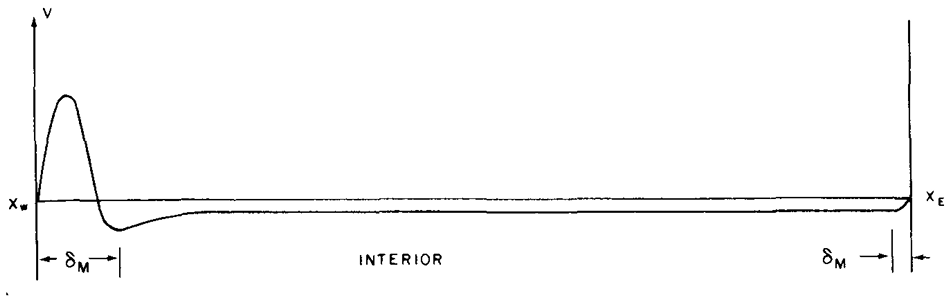
\includegraphics[width=1.00\textwidth]{assets/western_boundary_layer_velocity.png}
    \caption{西边界流的经向速度剖面}
    \label{fig:western_boundary_layer_velocity}
\end{figure}

根据Sverdrup平衡关系 \eqref{eq:sverdrup_balance}，内区流函数 $\streamfunc_0$ 可以通过对风应力旋度积分得到:
\begin{equation*}
    \streamfunc_0(x, y) = \int_{x_E}^{x} \kvec \cdot (\nabla_h \times \wind) \dd{x^\prime} + \streamfunc_0(x_E, y) = -\int_{x}^{x_E} \kvec \cdot (\nabla_h \times \wind) \dd{x^\prime}
\end{equation*}

特别地，在西边界层的外缘 (即内区的西部边界 $x=x_W$)，内区流函数的值为:
\begin{equation}
    \streamfunc_0(x_W, y) = -\int_{x_W}^{x_E} \kvec \cdot (\nabla_h \times \wind) \dd{x'}
    \label{eq:interior_transport_total}
\end{equation}

上式右端的物理含义是\textbf{内区Sverdrup输运的总量}。
由于风应力旋度在副热带海域通常为负 (反气旋式)，故 $\streamfunc_0(x_W, y) > 0$。

\begin{insightbox}[Munk理论的物理图景]
    \begin{enumerate}
        \item \textbf{强流特征与质量守恒}:
        西边界流的速度量级为 $O(\frac{\hscale}{\delta_M})$，远大于东边界流 $O(1)$ 的量级。
        可见，西边界流是一支极其强劲的窄流。
        物理上，这是质量守恒的必然要求: 广阔内区中缓慢向南的Sverdrup输运 ($\streamfunc_0(x_W, y)$)，必须通过狭窄边界层内的一支高速向北的流动完全补偿，从而形成闭合的水平环流。

        \item \textbf{流动的空间结构与回流}:
        西边界流经向速度解包含正弦项 $\sin(\frac{\sqrt{3}}{2}\lambda_W)$，具有显著的振荡特征。
        经向速度 $\flayer{v_0}$ 的零点由 $\sin(\frac{\sqrt{3}}{2}\lambda_W) = 0$ 决定。
        根据 $\lambda_W$ 的取值范围，流动呈现出多带结构:
        \begin{itemize}
            \item \textbf{主西边界流} ($0 < \lambda_W < \frac{2\pi}{\sqrt{3}}$):
            在此区间内 $\flayer{v_0} > 0$，流体向北高速流动。
            著名的例子是\textbf{湾流 (Gulf Stream)} 和\textbf{黑潮 (Kuroshino)}。

            \item \textbf{西边界回流} ($\frac{2\pi}{\sqrt{3}} < \lambda_W < \frac{4\pi}{\sqrt{3}}$):
            在此区间内 $\flayer{v_0} < 0$，流体向南流动。
            这表明在主西边界流的东侧外缘，理论上存在一支逆流，被称为\textbf{再循环流 (Recirculation)}。
        \end{itemize}
        理论成功地在定性上解释了实际观测中湾流东侧存在的再循环结构，体现了Munk理论的合理性。

        \item \textbf{维持平衡}:
        大洋西边界高速经向流动向北输送的质量通量精确抵消了风应力旋度在整个内区驱动的向南Sverdrup输运，从而维持了整个大洋盆地的质量平衡和涡度平衡。

        \item \textbf{动力学各向异性}:
        东西边界运动状态的差异反映了摩擦效应在物理空间中的非对称性。
        $\beta$ 效应使得涡度的动力学性质具有显著的各向异性。
    \end{enumerate}
\end{insightbox}
